
\chapter{Description de la passerelle}\label{ch:passerelle}

La passerelle est chargée du traitement des paquets reçu par les capteurs et du stockage de ces données dans la base de données. 

Elle se compose de deux parties physique, d'une part un module de gestion de la communication LoRa, le concentrateur, qui se charge de la réception des paquets radio LoRa. L'autre partie est le micro-ordinateur, lorsqu'un paquet de données est reçu par le concentrateur, l'ordinateur de traitement le récupère puis se charge de décoder les données pour ensuite les stocker.

La passerelle utilise une distribution du système d'exploitation Linux sur lequel sont exécutés deux programmes: le packet forwader et le serveur d'application.

Le packet forwarder est un logiciel qui a est disponible sur internet gratuitement, son but est de récupérer les messages LoRa reçus par le concentrateur et de transformer les paquets en messages de type json qui sont ensuite transmis au travers d'un socket sous la forme d'un paquet UDP.

Le serveur d'application qui a été développé spécialement pour le travail de Bachelor, est le programme qui se charge du traitement des paquets UDP envoyés par le packet forwarder. C'est lui qui est responsable d'extraire les données des strings json et de les stocker.

Afin de pouvoir respecter les contraintes de temps du TB, une seule passerelle sera assemblée pour le projet.

La figure \ref{fig:gateway_schema} présente le schéma block de la passerelle.

\section{Le matériel}

L'ordinateur de traitement des paquets LoRa se base sur le micro-ordinateur très connu Raspberry Pi. Il dispose de toute les ressources nécessaire pour les besoins du travail de Bachelor, de plus la communauté et la documentation à son sujet est très développée.

Pour rappel les caractéristiques du Raspberry Pi sont résumées dans la table~\ref{tab:raspberry_cara}.

\begin{table}[htb]
\caption{Caractéristiques du Raspberry Pi 3 Model B+}
\label{tab:raspberry_cara}
\centering
\begin{tabular}{ l | l }
\toprule
Dimensions & 85mm x 49mm \\
\midrule
Microcontrôleur & Broadcom BCM2837B0 – Cortex-A53 64-bit \\
\midrule
Oscillateur & 1.4 Ghz \\
\midrule
Stockage & Carte SD \\
\midrule
RAM & 1 GB SDRAM \\
\midrule
WiFi & 802.11 b/g/n/ac \\
\midrule
Prix & 34.50 CHF\\
\bottomrule 
\end{tabular}
\end{table}

Pendant la pré-étude deux concentrateurs différents avaient été étudié, le choix final c'est porté sur la solution d'un concentrateur moins couteux, le Dragino LoRa HAT. C'est un concentrateur de type simple canal, c'est à dire qu'il n'es capable d'écouter qu'une seule fréquence à la fois, ce qui convient parfaitement pour un prototype comme celui développé pour le projet puisque un seul capteur sera assemblé. Le Dragino LoRa HAT est un module d'extension pour la Raspberry Pi, il est conçu pour se fixer au dessus de lui aisément. En plus de la gestion de la couche radio LoRa le module propose également un module GPS qui pourrait se rendre intéressant pour déterminer la position des passerelles, cet axe pourrait être intéressant pour le développement d'un produit.

Pour rappel les caractéristiques du Dragino Hat sont résumées dans la table~\ref{tab:dragino_cara}.

\begin{table}[htb]
\caption{Caractéristiques du Dragino LoRa Hat}
\label{tab:dragino_cara}
\centering
\begin{tabular}{ l | l }
\toprule
Dimensions & 60mm x 53mm x 25mm \\
\midrule
LoRa & SX1276 \\
\midrule
Type de passerelle & Simple canal \\
\midrule
Prix & 38.90 CHF \\
\bottomrule
\end{tabular}
\end{table}

Le Raspberry Pi et le Dragino LoRa HAT communiquent au travers d'un bus de type SPI. La gestion de la communication est entièrement géré par le logiciel packet forwarder.

\begin{figure}[htb]
\centering 
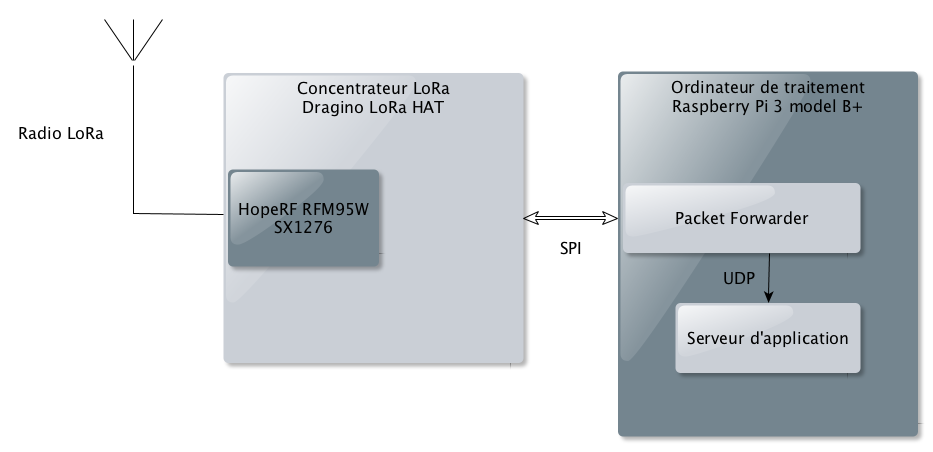
\includegraphics[width=0.8\columnwidth]{gateway_detailed_schema.png} 
\caption{Schéma block de la passerelle}
\label{fig:gateway_schema}
\end{figure}

\todo{Figure RPI + Dragino}

\section{Le packet forwarder}

Le packet forwarder est le logiciel qui se place en amont du serveur d'application, il est en charge de la gestion du Dragino LoRa HAT, c'est à dire qu'il va régulièrement interroger le module d'extension pour savoir si de nouveaux paquets sont disponibles, si c'est le cas, le packet forwarder va les récupérer en analyser le contenu afin de pouvoir créer une string json contenant toutes les informations. En plus de cela il va aussi rajouter des meta-données, comme le temps de réception du paquet ainsi que la fréquence et le facteur d'étalement par exemple.

Une fois le paquet transformé en objet json, le tout est envoyé au moyen d'un paquet UDP à un serveur, dans notre cas le serveur d'application. La liste suivante décrit les informations contenu dans le paquet.

\begin{itemize}
\item La version du protocole utilisée
\item Un jeton aléatoire utilisé pour marquer les paquets
\item Un identifiant du type de message
\item Un identifiant unique de la passerelle
\item L'objet json
\end{itemize}

Pour les paquets de type PUSH\_DATA, qui sont les seuls paquets utilisés dans le cadre du projet et qui sont créé pour les données du flux montant (noeud -> passerelle), l'objet json contient un tableau nommé rxpk. Chaque élément du tableau peut contenir les informations suivantes.

\begin{itemize}
\item time: Heure UTC à la réception du paquet
\item tmms: Temps GPS à la réception du paquet (nombre de ms depuis le 6 janvier 1980)
\item tmst: Temps interne de l'événement "RX finished"
\item freq: La fréquence centrale en Mhz à la réception
\item chan: Le canal de réception
\item rfch: La chaîne radio fréquence utilisée pour la réception
\item stat: Status du CRC du paquet (1 = OK, - 1 = NOK, 0 = Pas de CRC)
\item modu: Modulation LORA ou FSK
\item datr: Le taux de transfert LoRa (par exemple SF12BW500, facteur d'étalement 12, largeur de bande 500Mhz)
\item codr: Identifiant du taux LoRa ECC
\item rssi: RSSI (Received Signal Strength Indication) en dBm
\item lsnr: SNR (Signal to Noise Ratio) LoRa en dB
\item size: La taille en byte de la charge utile du paquet radio LoRa
\item data: La charge utile du paquet encodée en Base64
\end{itemize}

Un exemple d'objet json envoyé par le packet forwarder est présenté ci-dessous.

\todo{Mettre vrai exemple}

\begin{lstlisting}
{
	"rxpk":[
	{
		"time":"2013-03-31T16:21:17.528002Z",
		"tmst":3512348611,
		"chan":2,
		"rfch":0,
		"freq":866.349812,
		"stat":1,
		"modu":"LORA",
		"datr":"SF7BW125",
		"codr":"4/6",
		"rssi":-35,
		"lsnr":5.1,
		"size":32,
		"data":"-DS4CGaDCdG+48eJNM3Vai-zDpsR71Pn9CPA9uCON84"
	}
]}
\end{lstlisting}

Le protocole est décrit en grand détails sur la page github du packet forwarder de Semtech voir \cite{lora-pkt-forwarder-protocol}.

A la base le packet forwarder a été développé par la société Semtech, tenante de la patente du protocole de communication LoRa, c'est également cette société qui a définit le format des strings json envoyées dans les paquets UDP. Cependant la version qui est utilisée dans le cadre du projet de Bachelor, est un fork sur lequel plusieurs personnes ont travaillés afin de rajouter un certains nombre de fonctionnalité comme l'utilisation de fichiers de configuration ou le support de concentrateurs divers. Les principaux acteurs du développement de ce logiciel sont la société Semtech, Thomas Telkamp, Charles Hallard et Julien Le Sech. C'est le fork de Charles Hallard qui est employé par le projet car il supporte le Dragino LoRa HAT, il est disponible gratuitement sur github. \cite{pkt-forwarder-hallard}

Les tâches en lien avec le packet forwarer sont très simple, il s'agit d'abord de cloner le repository git puis de configurer le packet forwarder au moyen d'un fichier json, principalement pour sélectionner la fréquence et le facteur d'étalement sur lequel il doit écouter ainsi que l'adresse et le port du serveur auquel on souhaite envoyer les paquets UDP générés. On peut ensuite exécuter simplement le packet forwarder et dès la réception de paquets ils seront automatiquement transférés.

\section{Le serveur d'application}

Le serveur d'application est le logiciel principal de gestion de la passerelle. Au démarrage il se connect à un port du packet forwarder, ce qui lui permet ensuite de recevoir les paquets de données LoRa sous la forme d'objet json. D'autre part il va également gérer la connexion à la base données afin de pouvoir y sauver les données qui auront été extraites.

Afin de pouvoir aider au debug, le serveur d'application propose également un shell, dans lequel il est possible d'exécuter différente commandes afin d'acquérir des informations sur l'état du serveur, comme par exemple d'afficher toutes les positions GPS acquises.




